% This is "sig-alternate.tex" V2.1 April 2013
% This file should be compiled with V2.5 of "sig-alternate.cls" May 2012
%
% This example file demonstrates the use of the 'sig-alternate.cls'
% V2.5 LaTeX2e document class file. It is for those submitting
% articles to ACM Conference Proceedings WHO DO NOT WISH TO
% STRICTLY ADHERE TO THE SIGS (PUBS-BOARD-ENDORSED) STYLE.
% The 'sig-alternate.cls' file will produce a similar-looking,
% albeit, 'tighter' paper resulting in, invariably, fewer pages.
%
% ----------------------------------------------------------------------------------------------------------------
% This .tex file (and associated .cls V2.5) produces:
%       1) The Permission Statement
%       2) The Conference (location) Info information
%       3) The Copyright Line with ACM data
%       4) NO page numbers
%
% as against the acm_proc_article-sp.cls file which
% DOES NOT produce 1) thru' 3) above.
%
% Using 'sig-alternate.cls' you have control, however, from within
% the source .tex file, over both the CopyrightYear
% (defaulted to 200X) and the ACM Copyright Data
% (defaulted to X-XXXXX-XX-X/XX/XX).
% e.g.
% \CopyrightYear{2007} will cause 2007 to appear in the copyright line.
% \crdata{0-12345-67-8/90/12} will cause 0-12345-67-8/90/12 to appear in the copyright line.
%
% ---------------------------------------------------------------------------------------------------------------
% This .tex source is an example which *does* use
% the .bib file (from which the .bbl file % is produced).
% REMEMBER HOWEVER: After having produced the .bbl file,
% and prior to final submission, you *NEED* to 'insert'
% your .bbl file into your source .tex file so as to provide
% ONE 'self-contained' source file.
%
% ================= IF YOU HAVE QUESTIONS =======================
% Questions regarding the SIGS styles, SIGS policies and
% procedures, Conferences etc. should be sent to
% Adrienne Griscti (griscti@acm.org)
%
% Technical questions _only_ to
% Gerald Murray (murray@hq.acm.org)
% ===============================================================
%
% For tracking purposes - this is V2.0 - May 2012

\documentclass{sig-alternate-05-2015}
  \pdfpagewidth=8.5truein
  \pdfpageheight=11truein
  
\usepackage{listings}
\usepackage{color}
\definecolor{mygreen}{rgb}{0,0.6,0}
\definecolor{mygray}{rgb}{0.5,0.5,0.5}
\definecolor{mymauve}{rgb}{0.58,0,0.82}

\lstset{ %
  backgroundcolor=\color{white},   % choose the background color
  basicstyle=\footnotesize,        % size of fonts used for the code
  breaklines=true,                 % automatic line breaking only at whitespace
  captionpos=b,                    % sets the caption-position to bottom
  commentstyle=\color{mygreen},    % comment style
  escapeinside={\%*}{*)},          % if you want to add LaTeX within your code
  keywordstyle=\color{blue},       % keyword style
  stringstyle=\color{mymauve},     % string literal style
}

\begin{document}

% Copyright
\setcopyright{acmcopyright}
%\setcopyright{acmlicensed}
%\setcopyright{rightsretained}
%\setcopyright{usgov}
%\setcopyright{usgovmixed}
%\setcopyright{cagov}
%\setcopyright{cagovmixed}


% DOI
\doi{http://dx.doi.org/xx.xxxx/xxxxxxx.xxxxxxx}

% ISBN
\isbn{978-1-4503-3739-7/16/04}

%Conference
%\conferenceinfo{PLDI '13}{June 16--19, 2013, Seattle, WA, USA}

\acmPrice{\$15.00}

%
% --- Author Metadata here ---
\conferenceinfo{SAC'16,}{ April 4-8, 2016, Pisa, Italy}
\CopyrightYear{2016} % Allows default copyright year (20XX) to be over-ridden - IF NEED BE.
%\crdata{0-12345-67-8/90/01}  % Allows default copyright data (0-89791-88-6/97/05) to be over-ridden - IF NEED BE.
% --- End of Author Metadata ---

\title{An Empirical Assessment of the Adoption of Java Generics and Lambda Expressions} 

% \subtitle{[Extended Abstract]
%
% You need the command \numberofauthors to handle the 'placement
% and alignment' of the authors beneath the title.
%
% For aesthetic reasons, we recommend 'three authors at a time'
% i.e. three 'name/affiliation blocks' be placed beneath the title.
%
% NOTE: You are NOT restricted in how many 'rows' of
% "name/affiliations" may appear. We just ask that you restrict
% the number of 'columns' to three.
%
% Because of the available 'opening page real-estate'
% we ask you to refrain from putting more than six authors
% (two rows with three columns) beneath the article title.
% More than six makes the first-page appear very cluttered indeed.
%
% Use the \alignauthor commands to handle the names
% and affiliations for an 'aesthetic maximum' of six authors.
% Add names, affiliations, addresses for
% the seventh etc. author(s) as the argument for the
% \additionalauthors command.
% These 'additional authors' will be output/set for you
% without further effort on your part as the last section in
% the body of your article BEFORE References or any Appendices.

\numberofauthors{8} %  in this sample file, there are a *total*
% of EIGHT authors. SIX appear on the 'first-page' (for formatting
% reasons) and the remaining two appear in the \additionalauthors section.
%
\author{
% You can go ahead and credit any number of authors here,
% e.g. one 'row of three' or two rows (consisting of one row of three
% and a second row of one, two or three).
%
% The command \alignauthor (no curly braces needed) should
% precede each author name, affiliation/snail-mail address and
% e-mail address. Additionally, tag each line of
% affiliation/address with \affaddr, and tag the
% e-mail address with \email.
%
% 1st. author
\alignauthor
Daniella Angelos\\
       \affaddr{Computer Science Department}\\
       \affaddr{University of Bras\'{i}lia}\\
       \affaddr{Bras\'{i}lia, Brazil}\\
% 2nd. author
\alignauthor
Thiago Cavalcanti\\
        \affaddr{Computer Science Department}\\
       \affaddr{University of Bras\'{i}lia}\\
       \affaddr{Bras\'{i}lia, Brazil}
% 3rd. author
\alignauthor Vin\'{i}cius Correa\\
       \affaddr{Computer Science Department}\\
       \affaddr{University of Bras\'{i}lia}\\
       \affaddr{Bras\'{i}lia, Brazil}
\and  % use '\and' if you need 'another row' of author names
% 4th. author
\alignauthor Rodrigo Bonif\'{a}cio\\
     \affaddr{Computer Science Department}\\
       \affaddr{University of Bras\'{i}lia}\\
       \affaddr{Bras\'{i}lia, Brazil}
}

\maketitle

\begin{abstract}
Modernizing legacy systems towards the evolution 
of the underlining programming language has been reported as 
a challenging task. For this reason, developers often prefer to maintain 
the use of existing constructs instead of using new language 
features. This scenario of language evolution might be well exemplified 
using two remarkable releases of Java programming language--- Java SE 5.0 (2004) 
and Java SE 8 (2014), for instance, in which considerable language 
improvements were proposed. Java SE 5.0 introduced parametric polymorphism to the language (using Java Generics) and Java SE 8 introduced Lambda Expressions. In this paper we empirically investigate the adoption of both features by considering 
open-source Java systems. In the case of Java Generics, differently 
from existing reasearch works, we compare the adoption of this 
language feature by considering two distinct groups. In the first group we 
only consider systems whose initial development 
started before the release of Java SE 5.0. In the second group we consider systems whose initial development started at least five years after the release of Java 
SE 5.0. In the case of Lambda Expressions, we contribute as one the first attempts to empirically characterize  the common usage of that language construct. Our results reveal that\ldots
% Has past decade since a significantly comportment concept was introduced in Java, Generics has been a power full accept that permit generalize many compartments between class and methods This work has like principal focus discovery how the community of developers has been comported about generics. Now is a good time to answer like teams has developer thus software. As means objective of this research is make a study to response how is created parametrizades class, attribute and methods or only teams using implementation generics based in support provide  by API and there are the possibility that abstain of create generics by many other circumstances such the support provide to library has a good quality  to concern new parametrizades constructions.\\
% By the way, we has a new concept about comportment in java that are lambda expressions, 
% that provide functional benefits in a OO language. Like lambda has new style to think, we want understand how is a behavior of teams using this concept and confront between two concepts to check a real benefit to softwares.\\
% \textbf{Q1: How is adoption lambda expressions by developers?}\\
% \textbf{Q2: How ware adoption generics in softwas before and after 2010?}\\

% It was about a decade ago that a significantly behavioral concept was introduced in Java: Generics. It has been a powerful tool that permits to generalize classes and to abstract over types. This work has as main focus, to discover how the community of developers has been incorporating this feature. Now is a good time to answer this question due to the time that has passed since it was first introduced, ie, softwares development that started before, technically, already had time to incorporate it, and a large number of new softwares has been added to the community since then.
% As a secondary goal of this research, we embrace a recent new feature of Java called lambda expressions, that provides functional benefits in an oriented object language based on lambda-calculus. Lambda-calculus requires a different way of thinking a solution, therefore, we wish to understand how teams of developers are using this new concept and check if it has real benefits to softwares.

\end{abstract}


%
% The code below should be generated by the tool at
% http://dl.acm.org/ccs.cfm
% Please copy and paste the code instead of the example below. 
%
\begin{CCSXML}
<ccs2012>
 <concept>
  <concept_id>10010520.10010553.10010562</concept_id>
  <concept_desc>Computer systems organization~Embedded systems</concept_desc>
  <concept_significance>500</concept_significance>
 </concept>
 <concept>
  <concept_id>10010520.10010575.10010755</concept_id>
  <concept_desc>Computer systems organization~Redundancy</concept_desc>
  <concept_significance>300</concept_significance>
 </concept>
 <concept>
  <concept_id>10010520.10010553.10010554</concept_id>
  <concept_desc>Computer systems organization~Robotics</concept_desc>
  <concept_significance>100</concept_significance>
 </concept>
 <concept>
  <concept_id>10003033.10003083.10003095</concept_id>
  <concept_desc>Networks~Network reliability</concept_desc>
  <concept_significance>100</concept_significance>
 </concept>
</ccs2012>  
\end{CCSXML}

\ccsdesc[500]{Computer systems organization~Embedded systems}
\ccsdesc[300]{Computer systems organization~Redundancy}
\ccsdesc{Computer systems organization~Robotics}
\ccsdesc[100]{Networks~Network reliability}


%
% End generated code
%

%
%  Use this command to print the description
%
\printccsdesc

% We no longer use \terms command
%\terms{Theory}

\keywords{Java Generics; lambda expressions; language evolution}

\section{Introduction}
Programming languages have to evolve to better address both techonology 
trends and developers needs. For instance, the Java programming language, which might be 
considered a reasonably recent language, presents features and constructs that 
differ significantly from its initial release in 1996. This kind of 
language evolution leads to a lot of dicussion regarding 
how this changes are embraced, used in practice, or ignored by the community of 
developers~\cite{}. One significant change to the Java language was 
the introduction of parametric polymorphism using Java Generics in 2004, which 
provides larger support for classes and methods generalization as well as 
improved support for software evolution. At that time, Java Generics 
was considered a significant improvement because it would simplify 
software construction by allowing the design of generic behavior using 
parametric types.

Several years later, Parnin et al. carried out an investigation to understand 
how Java Generics had been adopted in practice~\cite{}. 
In their study, they found out that over half of the projects and developers did not use generics at that time, and for those that did, the use was consistently narrow. They discovered, empirically, that generics were almost entirily used to either hold or traverse collections of objects in a type safe manner. 
%They concluded that an introduction of a language feature alone is not enough to assure adoption.
Nevertheless, the mentioned work did not answer a relevant question: is there 
any difference in the adoption of Java Generics when comparing two 
groups of systems based on the release date of this feature: one group of 
projects whose development started before Java SE 5.0 and one group of projects whose initial releases started after Java SE 5.0? 
{\color{red}Answering to this question might give \ldots}.

In this paper we first replicate the work of 
Pet et al.~\cite{} trying to answer aditional research questions~\ref{}. 

More recently, in 2014 a new version of the Java language was released (Java SE 8), introducing a long-waited feature that addresses some 
(limited) support for functional programming mechanisms: Lambda Expressions. In this paper we also characterize the adoption of that 
Java programming language construct, which might guide software 
developers to better understand the most common situations 
where Lambda Expressions should be used. In summary, the contributions of this paper are two-fold

\begin{itemize}
\item We replicate an existing study that investigates the 
adoption of Java Generics in open-source systems~\cite{}. Differently from 
the original work~\cite{}, our research also aims at 
understanding whether developers of recently developed 
systems embrace the use of Generics more extensively 
than developers of fully developed systems---whose initial 
releases started several years before Sun Microsystems 
launched Java SE 5.0 in 2004. 


\item We characterize how Java developers are using Lambda Expressions, 
a new Java language construct introduced in 2014 (Java SE 8). To 
the best of our knowledge, there is no other empirical study that investigates this issue.
\end{itemize}

\emph{Roadmap.} The remaining of this paper is organized 
as follows. {\color{red}In the next section \ldots} 
%At first, we investigate how programmers are adopting Generics, thus we did a deep study to try understand if this feature has been only used above API provided from oracle or if there is more audacious cases in which programmers has a real necessity to generalize behavior using generics to improve quality and simplicity of software.

% Actually in Java Language Specification (JSL8), oracle allowed mergin between paradigms. Java 8 that permit use lambda expression in construction OO, but how this comportamental featura has been adopted by community, maybe like occur with generics we want study how programmes has comportated to use functional programation inside a language OO.

% Here, we take look before and after 2010 to show how developers has been adopted estruturees using generics and  

%As the language continues to evolve, Java, in its 8th release, introduced a new construction that is the focus of the second goal of our research: lambda expressions. This feature provides functional benefits based on lambda-calculus and we aim to investigate, even little time had passed since the introduction of it, if it has been used by developers as oportunities to eliminate anonymous classes.

%This paper examines how software has been developed, to answer questions about generics and lambda expression using open source projects that has large impact in the community. We aim to contribute in the following aspects:
%\begin{itemize}
%\item We investigate claims about the adoption of Java Generics in softwares that started their developments after the Java release that integrated Generics.
%\item 
%\end{itemize}

%Like one of goal to explain how community only has been use api of generics in large %scale. Another question is about lambda function that like oracle ensure decrease %number of anonymous class and types that composite a software.\\
%Based in this question we choose 20 softwares with large adoption o commutity to focus %in quality of results.\\
%In results we waiting answer this 2 questions about the goal that language java %adopted in the new cenary to  


\section{Overview}

\subsection{Generics}
In 2004 Sun Microsystems introduced generics in benefit to remove ambiguity in collections like not specify the type and not doing so much cast in the collections.
Elimination of casts. The following code snippet without generics requires casting:

\begin{lstlisting}[language=java]
List list = new ArrayList();
list.add("hello");
String s = (String) list.get(0);
\end{lstlisting}

When re-written to use generics, the code does not require casting:

\begin{lstlisting}[language=java]
List<String> list = new ArrayList<String>();
list.add("hello");
String s = list.get(0);   // no cast
\end{lstlisting}

\subsection{Lambda}
	Like intent to help write a better code \textit{Java 8}. A significantly change focus in Collection API with addition of \textit{Streams} that allow us to write a better code about collections-processing at a hight level of abstraction. A good solution provide for \textit{Stream} is a trouble about concurrency that solve this with simple loops for and while was necessary a hard work and many boilerplate while \textit{parallelStream} is a elegant way to this.\\
	
	The difference between \textit{Collection} and \textit{Stream} is that \textit{Collection} is an data structure in memory while \textit{Stream}is a conceptually fixed data structure that computed elements by demand. When we using \textit{Collection Interface} require iteration provide by user while \textit{Stream Interface} uses internal iteration. Such as real example extracted Jetty 9.3.0:\\

	\begin{lstlisting}[language=java]
	List<String> actual = new ArrayList<>(); 
	for (Path path:finder.getHits()){
	 actual.add(hb.toShortForm(path.toFile()));
	}
	
	List<String> actual = finder.getHits().stream().map(hb.toShortForm(Path::toFile)).collect(toList());
	
	for(String parent:module.getParentNames()){
	 System.out.printf("Depend:%s%n",parent);
	}
	
	module.getParentNames().stream().forEach(parent->System.out.printf("Depend:%s%n",parent));
\end{lstlisting}

Based in this examples we have interested to research cases like this to find real opportunities of refactoring to prove that a adoption lambda expression in Java projects wold be a simple way to re-write a code and discovery if community has adopted Lambda to create a better code.\\
Like this we have 2 questions about lambda to guide this work:
\textbf{RQ1:} How was adoption of Lambda by the community?\\
\textbf{RQ2:} There are any construction with Lambda in a projects?\\


\section{Related work}
After a release of new language feature, manifold studies are published related to use and benefits of it. This section gives an overview of researches about Generics and Lambda Expression.

\subsection{Generics claims and empirical studies}

There are two basic types of works about Generics, the first one explore claims about its use in several contexts, and the benefits it brings. The second type performs empirical studies and tries to verify the claims and hypothesis made by some of the articles in the first type.
As the question we want answered is related to the use of this feature by developers a decade after its release, we'll give a breef only in a few works on empirical study.

{\color{blue} mencionar Mining Billions of AST Nodes to Study Actual and
Potential Usage of Java Language Features }

The aforementioned \textit{ 
Java Generics Adoption: How New Features are
Introduced, Championed, or Ignored
} empirical study about the use of Generics in open source communities is the main result we have related to Java Generics use until now. Several claims were tested in 20 ``most used'' projects at that time, but their focus were only in three of these projects: JEDIT, ECLIPSE-CS and SQUIRREL-SQL.
Their study concluded that Generics wasn't being used in a relevant manner.
{\color{blue} mencionar outros estudos que citam este trabalho }.
Our goal is to replicate part of this study and avaliate if, even a few years later, the use of Generics is still restricted to either hold or traverse collections of objects in a type safe manner, or if developers are using it more broadly.

\subsection{Lambda Expressions}

%We found only a few works related to Java Lambda Expressions in our research, and they are focused in measuring performance of this feature~\cite{} or making comparisons with Scala constructs~\cite{}, among others. But none of these works investigates real adoption of Lambda Expressions by developers.

%In our reserch, we found some work related to the use of lambda expressions in Java, focusing in comparisons with constructions in Scala Language cite(work\_lambda1) , efficiency gains cite(work\_lambda2), etc but none of this works investigating real adoption in projects.




\section{Investigation}

\subsection{Projects studied}

We choose 27 open source projects with the last public release in 2015. Here are we choose \textit{Ant}, \textit{Hibernate orm}, \textit{Openmeetings}, \textit{Tomcat}, \textit{Archiva}, \textit{Jclouds}, \textit{Platform Community}, \textit{UniversalMediaServer}, \textit{Bonita-Tools}, \textit{Jenkins},\textit{Postgree jdbc}, \textit{Wicket},\textit{Cassandra}, \textit{Jmeter}, \textit{Sonar}, \textit{Wildfly},\textit{Checkstyle}, \textit{Log4j}, \textit{Spark}, \textit{Woden}, \textit{Crawler4j} ,\textit{Maven}, \textit{Spring}, \textit{Zookeeper},\textit{Eclipse}, \textit{MyFaces} and \textit{Storm} we choose this because are constantly update and has a large adoption on open source community.\\ 


%We choose 6 open source projects, \textit{Hibernate}, \textit{Jasper}, \textit{JBPM JBoss}, \textit{Jetty}, \textit{Tomcat} and \textit{Maven}, that has large adoption and contribution inside the open source community. All these projects have many releases and large historic of updates that possibility a deep analysis to investigation in view of the releases followed by all features that was appeared in Java language.



\subsection{Methodology}
We start doing static analyzing in all \textit{.java} files in open source projects that we choose, to collected data around how often the community generics and lambda expressions at the time was generated an AST to each file source. Based on structure and abstraction provided from Eclipse JDT we choose this API to support generates a parse tree to each file and creation of each visitor \cite{Gamma:1995:DPE:186897}. We choose to use the framework Spring to inject the visitors such as dependence. Therefore like an ideal configuration in visitor \cite{Gamma:1995:DPE:186897} when found a ideal construction as base from this paper, this is save to analysis with R language \cite{R}.\\

The Static Analyses has a visitor to search  Lambda Expression because we have a intent to discovery how community has been accepted this feature so waited. Another hand, we cant leave explain how community has ignored an opportunity to make a simple refactoring in large scale when not use Lambda to replace a Enhanced For to iterate a Collection. Like it each occur of Lambda Expression and Enhanced For are save in a csv file to analysis marking source file and line of start and project name end of each construction founded.\\
  

\section{Results}

\subsection{Lambda}
After analysis around 3.5M LOC, we founded 438 cases to Lambda inside unit test. We concluded that a large use in unit test probability because developers work with anonymous methods provide for Lambda and to increase a productive and isn't necessary create methods to make tests.\\

\begin{figure}[h]
	\center
	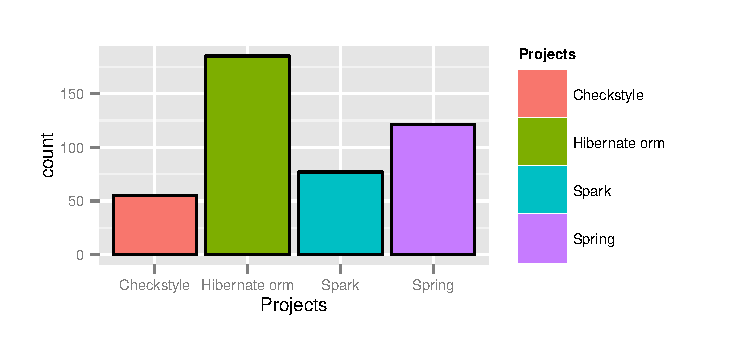
\includegraphics[width=0.60\textwidth]{lambdaTest}
	\label{fig:testsLambda}
	\caption{Use of Lambda in unit tests.}
\end{figure}

Another relevant point is that developers ignore a real opportunities to refactoring iteration in Collections with Stream and prefer use \textit{Enhanced For} to do it. In this research we founded 18821 cases in 23 projects to convert \textit{Enhanced For} to \textit{Stream} interface provide that avoid some boilerplate and open opportunities to do concurrency in Collections through \textbf{parallelStream}, in figure ~\ref{fig:opportunitiesLambda} occur about Enhanced.\\

\begin{figure}[h]
	\center
	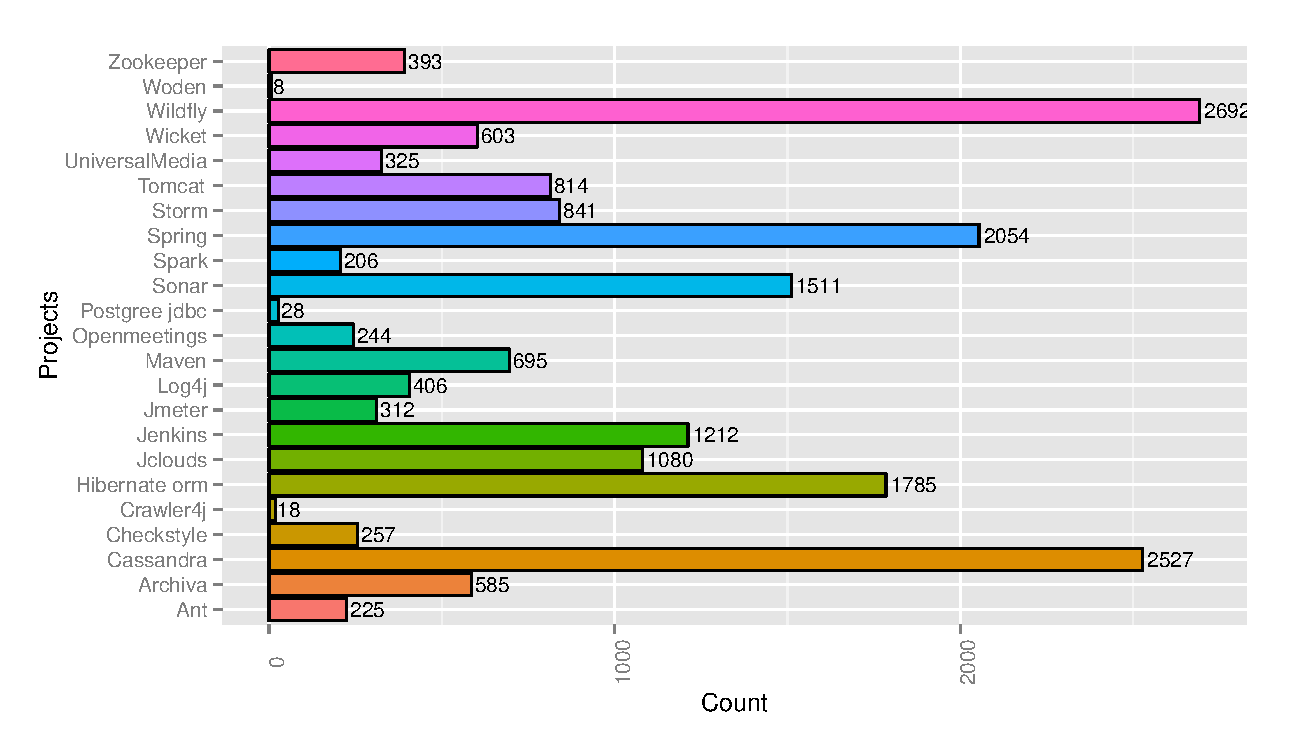
\includegraphics[width=0.55\textwidth]{lamdaOpport}
	\label{fig:opportunitiesLambda}
	\caption{Oportunites to replace For by Lambda.}
\end{figure}




\section{Future work}
Generics ????\\

Maybe with a large adoption of community for lambda become possible the the use of language Scale was increased. However that a paradigm function was incorporated in Java and was a good work discovery if it can replace constructors in Scala. Another point is that Lambda provide solution more elegant to concurrency in a loop avoid boilerplate and generated a construct more clear but the big problems is how test Lambda Expression with a elegant form showed this construction are anonymous methods. \\



%ACKNOWLEDGMENTS are optional
\section{Acknowledgments}
This section is optional; it is a location for you
to acknowledge grants, funding, editing assistance and
what have you.  In the present case, for example, the
authors would like to thank Gerald Murray of ACM for
his help in codifying this \textit{Author's Guide}
and the \textbf{.cls} and \textbf{.tex} files that it describes.

%
% The following two commands are all you need in the
% initial runs of your .tex file to
% produce the bibliography for the citations in your paper.
\bibliographystyle{abbrv}
\bibliography{sigproc}  % sigproc.bib is the name of the Bibliography in this case
% You must have a proper ".bib" file
%  and remember to run:
% latex bibtex latex latex
% to resolve all references
%
% ACM needs 'a single self-contained file'!
%
%APPENDICES are optional
%\balancecolumns
\appendix
%Appendix A
\section{Headings in Appendices}
The rules about hierarchical headings discussed above for
the body of the article are different in the appendices.
In the \textbf{appendix} environment, the command
\textbf{section} is used to
indicate the start of each Appendix, with alphabetic order
designation (i.e. the first is A, the second B, etc.) and
a title (if you include one).  So, if you need
hierarchical structure
\textit{within} an Appendix, start with \textbf{subsection} as the
highest level. Here is an outline of the body of this
document in Appendix-appropriate form:
\subsection{Introduction}
\subsection{The Body of the Paper}
\subsubsection{Type Changes and  Special Characters}
\subsubsection{Math Equations}
\paragraph{Inline (In-text) Equations}
\paragraph{Display Equations}
\subsubsection{Citations}
\subsubsection{Tables}
\subsubsection{Figures}
\subsubsection{Theorem-like Constructs}
\subsubsection{A Caveat for the \TeX\ Expert}
\subsection{Conclusions}
\subsection{Acknowledgments}
\subsection{Additional Authors}
This section is inserted by \LaTeX; you do not insert it.
You just add the names and information in the
\texttt{{\char'134}additionalauthors} command at the start
of the document.
\subsection{References}
Generated by bibtex from your ~.bib file.  Run latex,
then bibtex, then latex twice (to resolve references)
to create the ~.bbl file.  Insert that ~.bbl file into
the .tex source file and comment out
the command \texttt{{\char'134}thebibliography}.
% This next section command marks the start of
% Appendix B, and does not continue the present hierarchy
\section{More Help for the Hardy}
The sig-alternate.cls file itself is chock-full of succinct
and helpful comments.  If you consider yourself a moderately
experienced to expert user of \LaTeX, you may find reading
it useful but please remember not to change it.
%\balancecolumns % GM June 2007
% That's all folks!

\bibliographystyle{plain}
\bibliography{references.bib}


\end{document}